\chapter{Methodology}
\label{ch:methodology}

This section formalises the AI subsystem. We describe the overall topology (\S\ref{sec:topology}), present six algorithms in pseudocode (\S\ref{sec:algo-a1}--\S\ref{sec:algo-a6}), tie them together in multimodal session orchestration (\S\ref{sec:orchestration}), and propose a multi-intent user representation (\S\ref{sec:multi-intent}) that addresses the single-vector limitation identified in the review.

\section{System Topology}
\label{sec:topology}

The runtime topology comprises five planes: the frontend (\texttt{sprout-web}, Next.js), the Gemini Proxy (Node.js on Cloud Run), the backend (\texttt{sprout-backend}, Firebase Cloud Functions), Firestore, and the Gemini Live API. Two key lines distinguish this topology from the legacy LiveKit-based one: (i) the frontend connects directly to the proxy over WebSocket, and (ii) the proxy connects directly to the Gemini Live API---there is no Cloud Function in the audio path.

\begin{figure}[H]
\centering
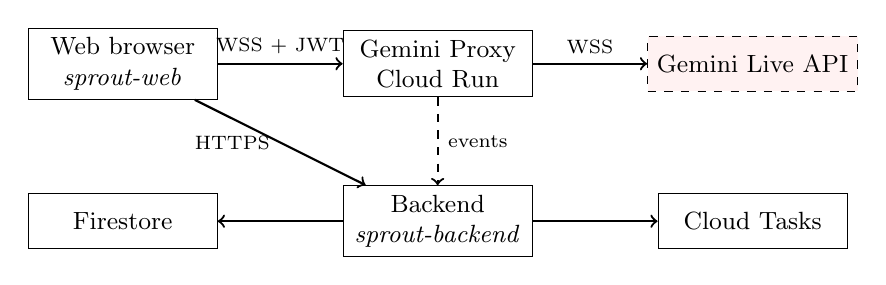
\begin{tikzpicture}[
    box/.style={rectangle, draw, minimum width=2.4cm, minimum height=0.7cm, align=center, font=\small},
    ext/.style={rectangle, draw, dashed, fill=red!5, minimum width=2.4cm, minimum height=0.7cm, align=center, font=\small},
    arrow/.style={->, thick}
]
\node[box] (web) at (0,2) {Web browser\\\textit{sprout-web}};
\node[box] (proxy) at (4,2) {Gemini Proxy\\Cloud Run};
\node[ext] (gemini) at (8,2) {Gemini Live API};
\node[box] (backend) at (4,0) {Backend\\\textit{sprout-backend}};
\node[box] (fs) at (0,0) {Firestore};
\node[box] (tasks) at (8,0) {Cloud Tasks};
\draw[arrow] (web) -- node[above, font=\scriptsize]{WSS + JWT} (proxy);
\draw[arrow] (proxy) -- node[above, font=\scriptsize]{WSS} (gemini);
\draw[arrow] (web) -- node[left, font=\scriptsize]{HTTPS} (backend);
\draw[arrow] (backend) -- (fs);
\draw[arrow] (backend) -- (tasks);
\draw[arrow, dashed] (proxy) -- node[right, font=\scriptsize]{events} (backend);
\end{tikzpicture}
\caption{Sprout AI runtime topology. The browser maintains WSS to the proxy (live data plane) and HTTPS REST to the backend (control plane).}
\label{fig:topology}
\end{figure}

\section{Algorithm A1: JWT-Validated Session Establishment}
\label{sec:algo-a1}

Algorithm~\ref{alg:a1} establishes a Gemini Live session. JWT verification follows the OpenID Connect profile: signature against JWKS, audience match, and expiry with a 5-second grace window. The JWT is passed as a URL query parameter because browser WebSocket clients cannot set custom headers. Banned-status is checked in real time against \texttt{users/\{uid\}.banned}.

\begin{algorithm}[H]
\caption{ValidateJwtAndOpenSession}
\label{alg:a1}
\begin{algorithmic}[1]
\Require Incoming WebSocket $c$ with query parameter \texttt{auth}
\Ensure Active session $s$ bound to $c$, or $c$ closed with status 4401
\State $jwt \gets c.\texttt{auth}$
\If{$jwt = \bot$} \State Close($c$, 4401); \Return \EndIf
\State $p \gets \textsc{VerifyJwt}(jwt, \text{audience})$
\If{$p = \bot$} \State Close($c$, 4401); \Return \EndIf
\If{\textsc{IsBanned}($p.\texttt{uid}$)} \State Close($c$, 4403); \Return \EndIf
\State $quota \gets \textsc{LookupQuota}(p.\texttt{uid})$
\If{$quota.\text{remaining} \leq 0$} \State Close($c$, 4429); \Return \EndIf
\State $ws_{\text{up}} \gets \textsc{OpenWebSocket}(\text{geminiLiveUrl})$
\If{$ws_{\text{up}} = \bot$} \State Close($c$, 4502); \Return \EndIf
\State $s \gets \textsc{NewSession}(p.\texttt{uid}, ws_{\text{up}}, c)$
\State \textsc{EmitEvent}(\texttt{session\_started}, $s$) \Comment{async to backend}
\State \Return $s$
\end{algorithmic}
\end{algorithm}

\section{Algorithm A2: Tokenised Message Routing}
\label{sec:algo-a2}

Algorithm~\ref{alg:a2} runs on each pipe (client$\rightarrow$upstream and upstream$\rightarrow$client). The proxy does not interpret audio or image frames; it accumulates token usage and batches persistence every 50 messages.

\begin{algorithm}[H]
\caption{RouteMessage (per pipe)}
\label{alg:a2}
\begin{algorithmic}[1]
\Require Session $s$, message $m$
\State $s.\texttt{lastActiveAt} \gets \textsc{Now}()$
\If{\textsc{IsRateLimited}($s.\texttt{uid}$)} \State \textsc{SendError}($s$, \texttt{rate\_limited}); \Return \EndIf
\If{$m$ contains \texttt{usageMetadata}}
    \State $s.\texttt{tokens.in} \mathrel{+}= m.\texttt{usageMetadata.prompt}$
    \State $s.\texttt{tokens.out} \mathrel{+}= m.\texttt{usageMetadata.response}$
\EndIf
\If{$m$ is a \texttt{function\_call}} \State \textsc{HandleFunctionCall}($s$, $m$)
\Else \State \textsc{Send}(\text{peer}, $m$) \EndIf
\State $s.\texttt{messageCount} \mathrel{+}= 1$
\If{$s.\texttt{messageCount} \bmod 50 = 0$} \State \textsc{Persist}($s$) \EndIf
\end{algorithmic}
\end{algorithm}

\section{Algorithm A3: Asynchronous Knowledge-Map Generation}
\label{sec:algo-a3}

Knowledge-map generation uses a two-phase pattern: synchronous enqueue ($\leq$250\,ms) and asynchronous worker ($\leq$60\,s). The \textsc{Sanitise} step rejects graphs exceeding 20 nodes, with cycles, or duplicate titles. \textsc{TopologicalRank} assigns layers for stable React Flow layout.

\begin{algorithm}[H]
\caption{GenerateKnowledgeMap}
\label{alg:a3}
\begin{algorithmic}[1]
\Require Skill query $q$, target level $\ell$, user $u$
\State $courseRef \gets \textsc{Firestore.Add}(\texttt{courses}, \{\texttt{status} := \texttt{pending}\})$
\State $taskId \gets \textsc{CloudTasks.Enqueue}(\texttt{kmapQueue}, \{courseId, q, \ell\})$
\State \Return $taskId$, $courseRef.\texttt{id}$
\State \textbf{Worker:} $G \gets \textsc{LlmGenerateGraph}(q, \ell)$
\State $G \gets \textsc{Sanitise}(G)$; $G \gets \textsc{TopologicalRank}(G)$
\State \textsc{Firestore.Update}($courseRef$, \{\texttt{knowledgeMap} := $G$, \texttt{status} := \texttt{ready}\})
\end{algorithmic}
\end{algorithm}

\section{Algorithm A4: Dual-Channel Lesson Completion Detection}
\label{sec:algo-a4}

Lesson completion is observed from agent side (dialogue mastery) and client side (navigation). Algorithm~\ref{alg:a4} uses client polling every 30\,s with idempotent agent-side writes.

\begin{algorithm}[H]
\caption{DetectLessonCompletion (client polling)}
\label{alg:a4}
\begin{algorithmic}[1]
\Require Lesson $\ell$, polling interval $\Delta = 30$\,s
\Loop
    \State $doc \gets \textsc{Firestore.Read}(\texttt{lessons}/\ell)$
    \If{$doc.\texttt{is\_completed}$} \State \textsc{Ui.ShowCompletionDialog}(); \textbf{break} \EndIf
    \State \textsc{Sleep}($\Delta$)
\EndLoop
\State \Comment{Agent-side:} \textsc{Firestore.Update}(\texttt{lessons}/$\ell$, \{\texttt{is\_completed} := \texttt{true}\})
\end{algorithmic}
\end{algorithm}

\section{Algorithm A5: Conversation Feedback Processing}
\label{sec:algo-a5}

After a session, feedback triggers summarisation and optional child-lesson generation gated by \textsc{ContainsConfusionMarkers}.

\begin{algorithm}[H]
\caption{OnConversationFeedbackUpdated}
\label{alg:a5}
\begin{algorithmic}[1]
\Require Conversation $c$ with feedback $f$
\State $transcript \gets \textsc{Firestore.ReadAll}(\texttt{conversations}/$c$/\texttt{messages})$
\State $summary \gets \textsc{LlmSummarise}(transcript)$
\State \textsc{Firestore.Update}($c$, \{\texttt{summary}\})
\If{$f.\texttt{rating} \leq$ thumbs-down \textbf{or} \textsc{ContainsConfusionMarkers}($summary$)}
    \State $topic \gets \textsc{ExtractWeakConcept}(summary)$
    \State \textsc{Firestore.Add}(\texttt{lessons}, \{\texttt{parentLessonId}, \texttt{title} := $topic$\})
\EndIf
\end{algorithmic}
\end{algorithm}

\section{Algorithm A6: Anonymous-to-Authenticated Progress Linking}
\label{sec:algo-a6}

\begin{algorithm}[H]
\caption{LinkAnonymousProgress}
\label{alg:a6}
\begin{algorithmic}[1]
\Require Authenticated UID $u_a$, anonymous account ID $a$, decision $\in \{\texttt{accept}, \texttt{decline}\}$
\If{decision = \texttt{decline}} \State mark $a$ for cleanup; clear cookie; \Return \EndIf
\For{each course $C$ in anonymous progress}
    \If{$C \notin$ authenticated progress} \State \textsc{Copy}($C$)
    \Else \State \textsc{MergeProgress}($C$) \Comment{union of completed lesson IDs}
    \EndIf
\EndFor
\State mark $a$ for cleanup; clear cookie
\end{algorithmic}
\end{algorithm}

\section{Multimodal Session Orchestration}
\label{sec:orchestration}

The six algorithms compose as follows: the user navigates to a lesson; the frontend opens the proxy WebSocket (Algorithm~\ref{alg:a1}); frames are exchanged (Algorithm~\ref{alg:a2}); polling watches completion (Algorithm~\ref{alg:a4}); feedback triggers summarisation (Algorithm~\ref{alg:a5}); anonymous users promote progress on sign-in (Algorithm~\ref{alg:a6}). No single algorithm holds the entire session in memory beyond the proxy's in-process map; Firestore holds the transcript; triggers perform post-session analysis.

\section{Multi-Intent User Representation}
\label{sec:multi-intent}

\textbf{Motivation.} The current design primes the tutor from \texttt{users/\{uid\}} (display name, job category) and a single conversation summary from Algorithm~\ref{alg:a5}. When a learner pursues multiple stylistically distinct interests (e.g.\ job interviews, cooking, and JavaScript), one summary collapses distinct intents---analogous to centroid collapse in multi-style recommendation~\cite{anh2026mmr}. The reviewer requested algorithmic detail for multi-interest personalization within the current architecture, not only as deferred future work.

\textbf{Schema extension.} We propose a subcollection \texttt{users/\{uid\}/course\_profiles/\{courseId\}} with fields:
\begin{itemize}
    \item \texttt{rollingSummary} (string, $\leq$512 tokens): concept-level summary updated by Algorithm~\ref{alg:a5} scoped to this course.
    \item \texttt{topics[]} (string[]): extracted weak/strong concepts from recent sessions.
    \item \texttt{masteryScore} (float $[0,1]$): aggregate completion and feedback signal.
    \item \texttt{lastActiveAt} (timestamp): recency for ranking.
    \item \texttt{embedding} (optional vector): for future ANN retrieval~\cite{malkov2018hnsw}.
\end{itemize}

\textbf{Context builder.} Algorithm~\ref{alg:context} replaces a single global summary with top-$k$ course profiles ($k=2$ by default) selected by recency and relevance to the active lesson.

\begin{algorithm}[H]
\caption{BuildSessionContext}
\label{alg:context}
\begin{algorithmic}[1]
\Require UID $u$, active \texttt{courseId}, \texttt{lessonId}
\State $profiles \gets \textsc{Firestore.Query}(\texttt{users}/$u$/\texttt{course\_profiles})$
\State $active \gets profiles[\texttt{courseId}]$
\State $candidates \gets$ sort $profiles \setminus \{active\}$ by \texttt{lastActiveAt} descending
\State $selected \gets \{active\} \cup$ top-$(k-1)$ from $candidates$ with $\texttt{masteryScore} > 0.3$
\State $ctx \gets$ merge(\texttt{display\_name}, \texttt{job\_category}, summaries from $selected$)
\State $ctx \gets ctx$ + lesson-specific prompt from \texttt{lessons/lessonId}
\State \Return $ctx$ \Comment{passed to Gemini system prompt, $\leq$ 1500 tokens}
\end{algorithmic}
\end{algorithm}

\textbf{Integration with A5.} When \textsc{OnConversationFeedbackUpdated} runs, the summary is written both to \texttt{conversations/\{id\}.summary} and to \texttt{course\_profiles/\{courseId\}.rollingSummary}, with \texttt{topics} and \texttt{masteryScore} updated incrementally. This is implementable without proxy changes: only Firestore triggers and prompt assembly in the backend change.

\textbf{Expected effect.} For learners with coherent single-course focus, behaviour is unchanged ($k=1$ effectively). For multi-course learners, the tutor receives distinct intent vectors rather than one averaged persona, improving personalization without waiting for multi-agent coordination (Section~\ref{sec:multi-agent}).
